\documentclass{tufte-handout}

\title{On ultimate; O1: primary middle, focus or left wing}
\author[James Reynolds]{James Reynolds}

%\date{28 March 2010} % without \date command, current date is supplied

%\geometry{showframe} % display margins for debugging page layout

\usepackage{graphicx} % allow embedded images
  \setkeys{Gin}{width=\linewidth,totalheight=\textheight,keepaspectratio}
  \graphicspath{{graphics/}} % set of paths to search for images
\usepackage{amsmath}  % extended mathematics
\usepackage{booktabs} % book-quality tables
\usepackage{units}    % non-stacked fractions and better unit spacing
\usepackage{multicol} % multiple column layout facilities
\usepackage{lipsum}   % filler text
\usepackage{fancyvrb} % extended verbatim environments
  \fvset{fontsize=\normalsize}% default font size for fancy-verbatim environments

% Standardize command font styles and environments
\newcommand{\doccmd}[1]{\texttt{\textbackslash#1}}% command name -- adds backslash automatically
\newcommand{\docopt}[1]{\ensuremath{\langle}\textrm{\textit{#1}}\ensuremath{\rangle}}% optional command argument
\newcommand{\docarg}[1]{\textrm{\textit{#1}}}% (required) command argument
\newcommand{\docenv}[1]{\textsf{#1}}% environment name
\newcommand{\docpkg}[1]{\texttt{#1}}% package name
\newcommand{\doccls}[1]{\texttt{#1}}% document class name
\newcommand{\docclsopt}[1]{\texttt{#1}}% document class option name
\newenvironment{docspec}{\begin{quote}\noindent}{\end{quote}}% command specification environment

\begin{document}

\maketitle% this prints the handout title, author, and date


\begin{marginfigure}%
  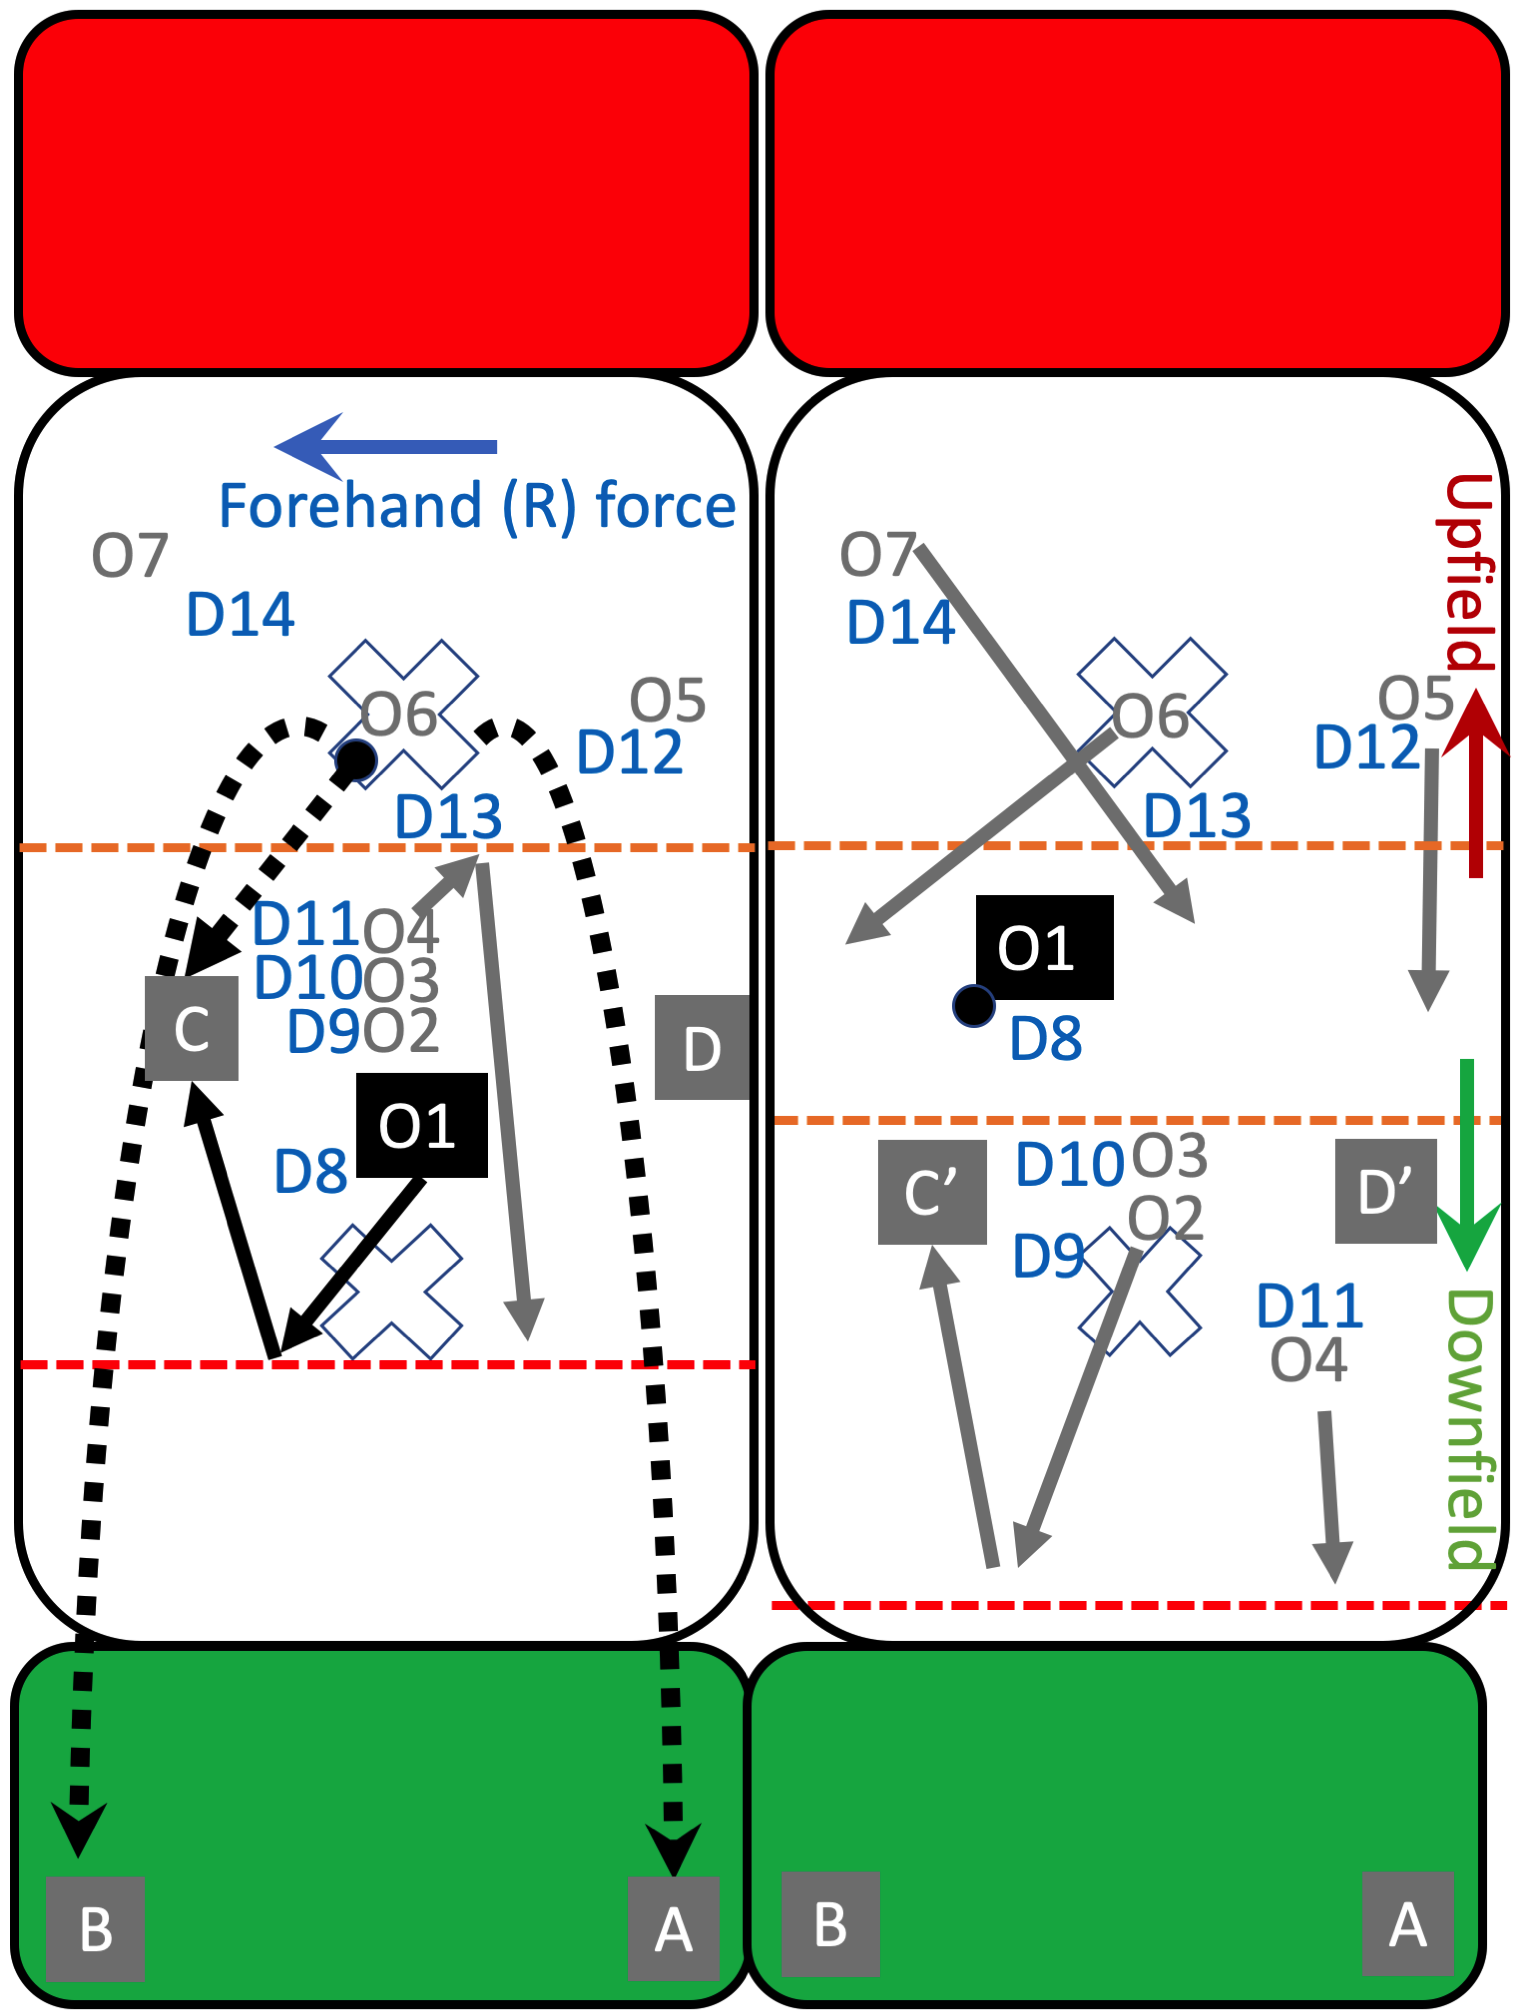
\includegraphics[width=\linewidth]{O1-vertical}
  \caption{Vertical stack formation}
  \label{fig:O1-vertical}
\end{marginfigure}



%\printclassoptions
This document is about 
playing primary 'middle', 
the focus, 
or left wing 
on offence,
referred to here 
as position O1\footnote{This
is part of a series, 
available at
\url{https://github.com/James-Reynolds/Ultimate-strategy-and-tactics}}.
You are starting the point on offence. 
Let the handlers 
deal with catching the pull, but
as you run downfield
try to 
see
what defence structure
is being used. 
%\footnote{It could be:
%person-match defence,
%person-match-last-back-helps,
%person-match-with-a-poacher,
%person-match-with-lots-of switching,
%force-middle,
%force-straight-up,
%zone-3-3-1-force-middle-
%zone-3-3-1-force-sideline
%zone-3-3-1-force-forehand
%zone-3-3-1-force-backhand
%zone-3-3-1-etc
%zone-3-2-2, 
%zone-2-3-2, 
%zone-1-3-2-1 (puppy-fence),
%clam,
%or something else}.

\section{Person-match defence: vertical stack}\label{sec:vertical}

Figure \ref{fig:O1-vertical} shows 
how everyone might 
setup 
if there is a brick called,
a forehand force, 
person-match defence, 
and a vertical stack.
Restricting your cutting 
to between 
the dashed 
horizontal 
lines 
can help\footnote{
Position of 
the dashed red line might vary
with how far O6 
can or will 
throw.}. 
If you go 
downfield of the dashed red line 
before the disc is in the air,
D8 may be able 
get to
A or B 
before the disc,
intercepting 
or preventing 
deep throws to 
you or others. 
Similarly, 
if you go 
upfield of the dashed yellow line
then D8 may 
be able to help
prevent dump throws from O6
to O5 
or O7.
Hence,
if you cut to C
but the disc is not thrown to you
perhaps cut deep 
to clear the area, 
then return to the stack
and make space for O2-O4. 


In Figure \ref{fig:O1-vertical} 
O6 is shown
potentially throwing 
you (O1) either:
\begin{enumerate}
\item A break-side 
huck to A.
This throw is 
probably 
difficult. 
However, you as O1
can just
stand still 
till O6 throws it, 
then run and catch it.
Figure \ref{fig:O1-vertical} indicates how 
D8 will be on the wrong side of you
and so probably 
be able to get to the disc
first.
\item An open-side huck to B. 
This is viable if: 
D8 is closer to the disc than you; 
you are faster than D8; or 
D8 does not cover 
an initial cut downfield (black arrow). 
\item A throw 
to C.
The solid black arrows indicate 
a cut you might do;
initially going deep,
but then coming back-under
on the open side.


\begin{marginfigure}%
  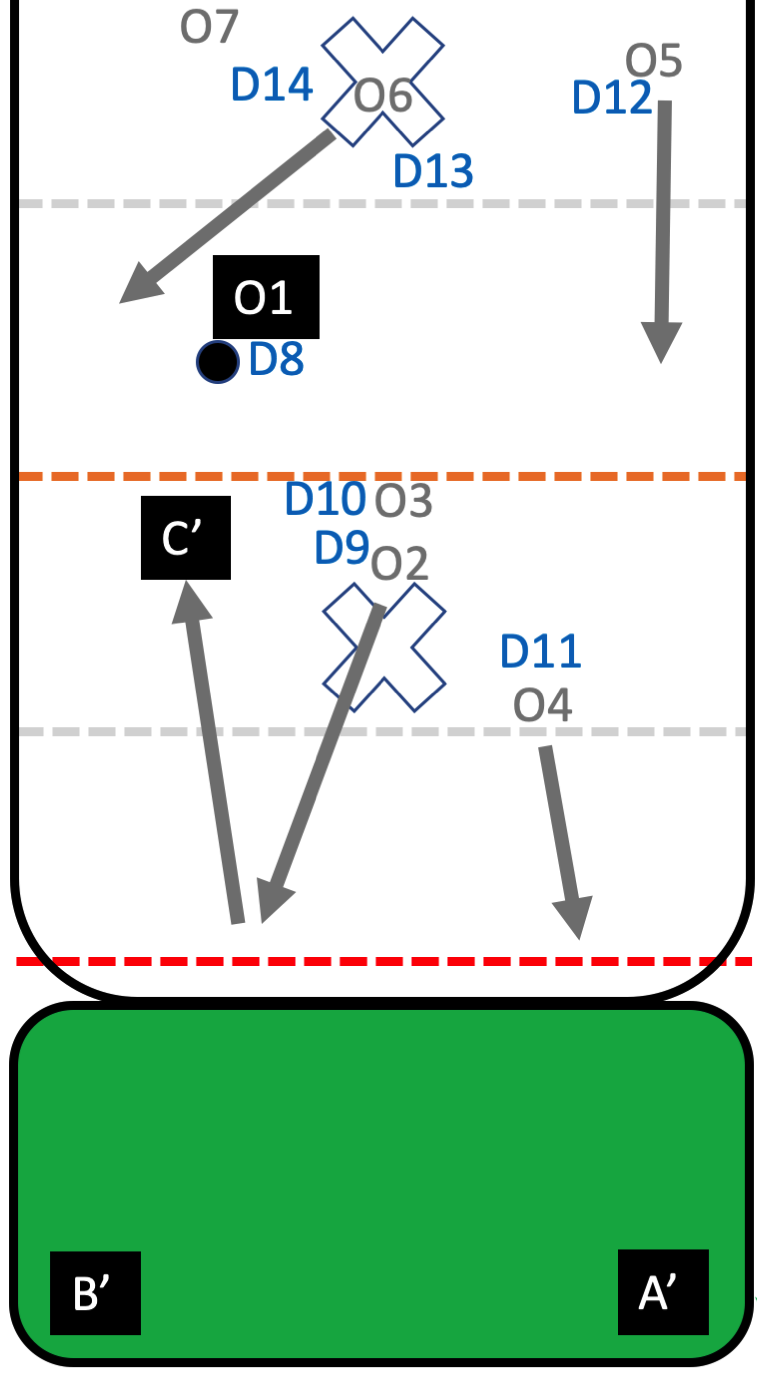
\includegraphics[width=\linewidth]{O1-vertical2}
  \caption{Vertical stack progression}
  \label{fig:O1-vertical2}
\end{marginfigure}




\item A break throw to D. 
Any of the cutters 
(O1-4)
can go and catch this, 
as all the defenders 
(D8-D11) 
are on the wrong side
However,
if anyone 
except O4 
cuts towards D 
prior to the disc being thrown 
then there is likely 
to be a pick\footnote{
Picks are
when a defender 
cannot follow 
someone they are marking.  
However, 
once the disc is thrown,
everyone can move anywhere 
to try and catch it. 
So, maybe stand still 
until it's thrown 
to avoid a pick}.
\end{enumerate}

Figure \ref{fig:O1-vertical2} shows 
the disc having been thrown to you
on the back-under cut towards C. 
In order of desirability, 
your options may include: 
(1)
off-load to O6, 
putting them in power position;
(2) throwing to A' to hit O2 or O4;
(3) throwing to B' or C' for O2;
(4) break force throw 
to centre the disc
to O3 or O5;
(5) dump to O7.
Then, head back to the stack, 
or make another cut.

%Vertical works
%for other person-match defences
%with adjustment\footnote{ 
%For example, 
%against (1) RH-backhand-force: mirror the above.
%against (2) person-match-straight-up-force: 
%hucks are likely harder, 
%but your defender (D8) 
%may just cover you under. 
%Hence, maybe just
%stand still as the handlers 
%move it around until
%they can send it deep.
%Otherwise, 
%maybe cut out to the sidelines}.


\subsection{Person-match defence: feldrunner offense}
\label{sec:feld}

\begin{marginfigure}%
  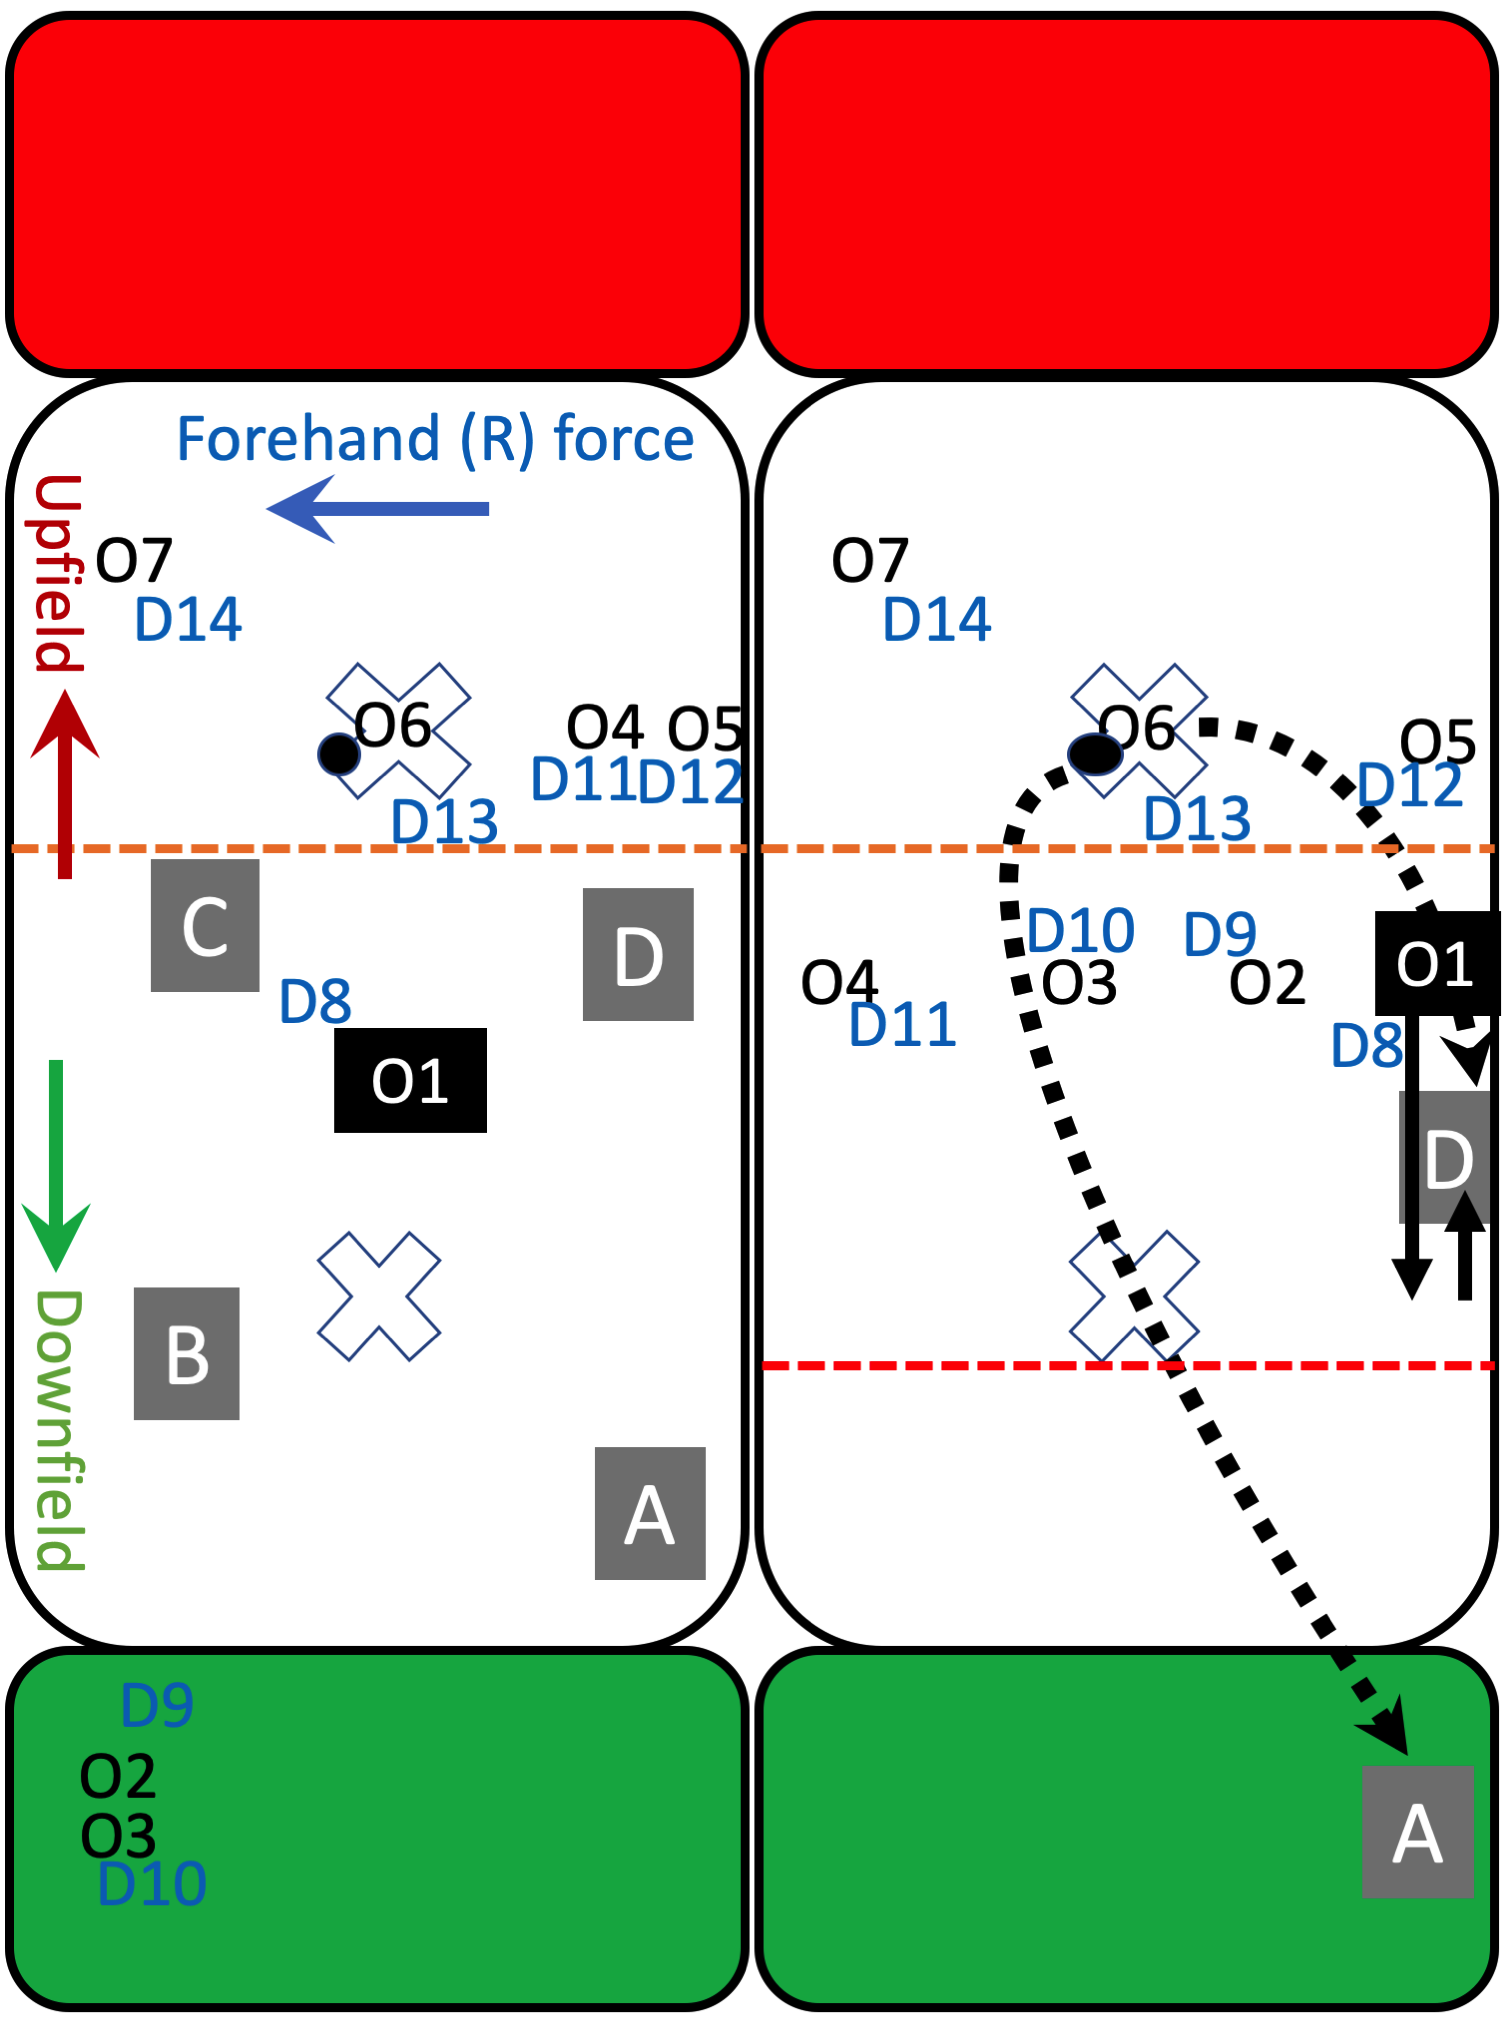
\includegraphics[width=\linewidth]{O1-horizontal}
  \caption{Feld (left) and ho-ro (right)}
  \label{fig:O1-horizontal}
\end{marginfigure}



Figure \ref{fig:O1-horizontal} (left) 
shows a feldrunner formation, 
with 4 handlers
and 2 in an 
endzone stack.
It involves 
leaving you 
(O1) 
isolated 
in the centre
as the focus. 
O6 can throw 
to A,
B, 
C 
or D. 
If D8 looks at you, 
let O6 throw it first. 
If D8 is 
looking at O6, 
make a cut. 
Once you get the disc 
either throw a goal 
to O2-3, 
or dump to 
one of O4-7 
and repeat. 


\subsection{Person-match defence: horizontal stack}\label{sec:horizontall}
Basic horizontal stack 
involves cutting
upfield and downfield (black arrows)
within your quarter of the field\footnote{
Other cuts
can work. 
For example, 
diamond cuts 
involve trading places 
with your neighbour
(02). 
However, this may need
coordination. 
So maybe keep it simple 
and just stay on the wing?}. 
Figure \ref{fig:O1-horizontal} (right) shows 
O1 on the left wing. 
O6 
can potentially 
throw to you 
at A 
or D\footnote{
Black arrows
show how a back-under cut 
opens space 
for this throw.}. 
However, 
O6 throwing to 
O2, O3 or O4  
may be easier. 
Hence,  
you may wish to 
wait and 
cut later. 
If you do get the disc 
at D 
a huck to 
A for O2 or 
to B for O4 
may be effective.
Otherwise, 
get it to the middle of the field 
with a dump to O5 or O6. 

A typical pattern
is that D8 (marking you)
will try to help 
D9, D10 and D11 
by poaching deep\footnote{
Even switching to person-match-but-last-person-covers-deepest defence}. 
To beat this: 
you can trade spots with O5;
you can move across to the open side, 
between D10 and O6; or 
stay still 
on the left wing,
so O6 can throw it 
straight to you\footnote{
Also effective
for zone offence
because you spread the field,
as discussed below.}.

\section{Zone offence}\label{sec:zone}

\begin{marginfigure}%
  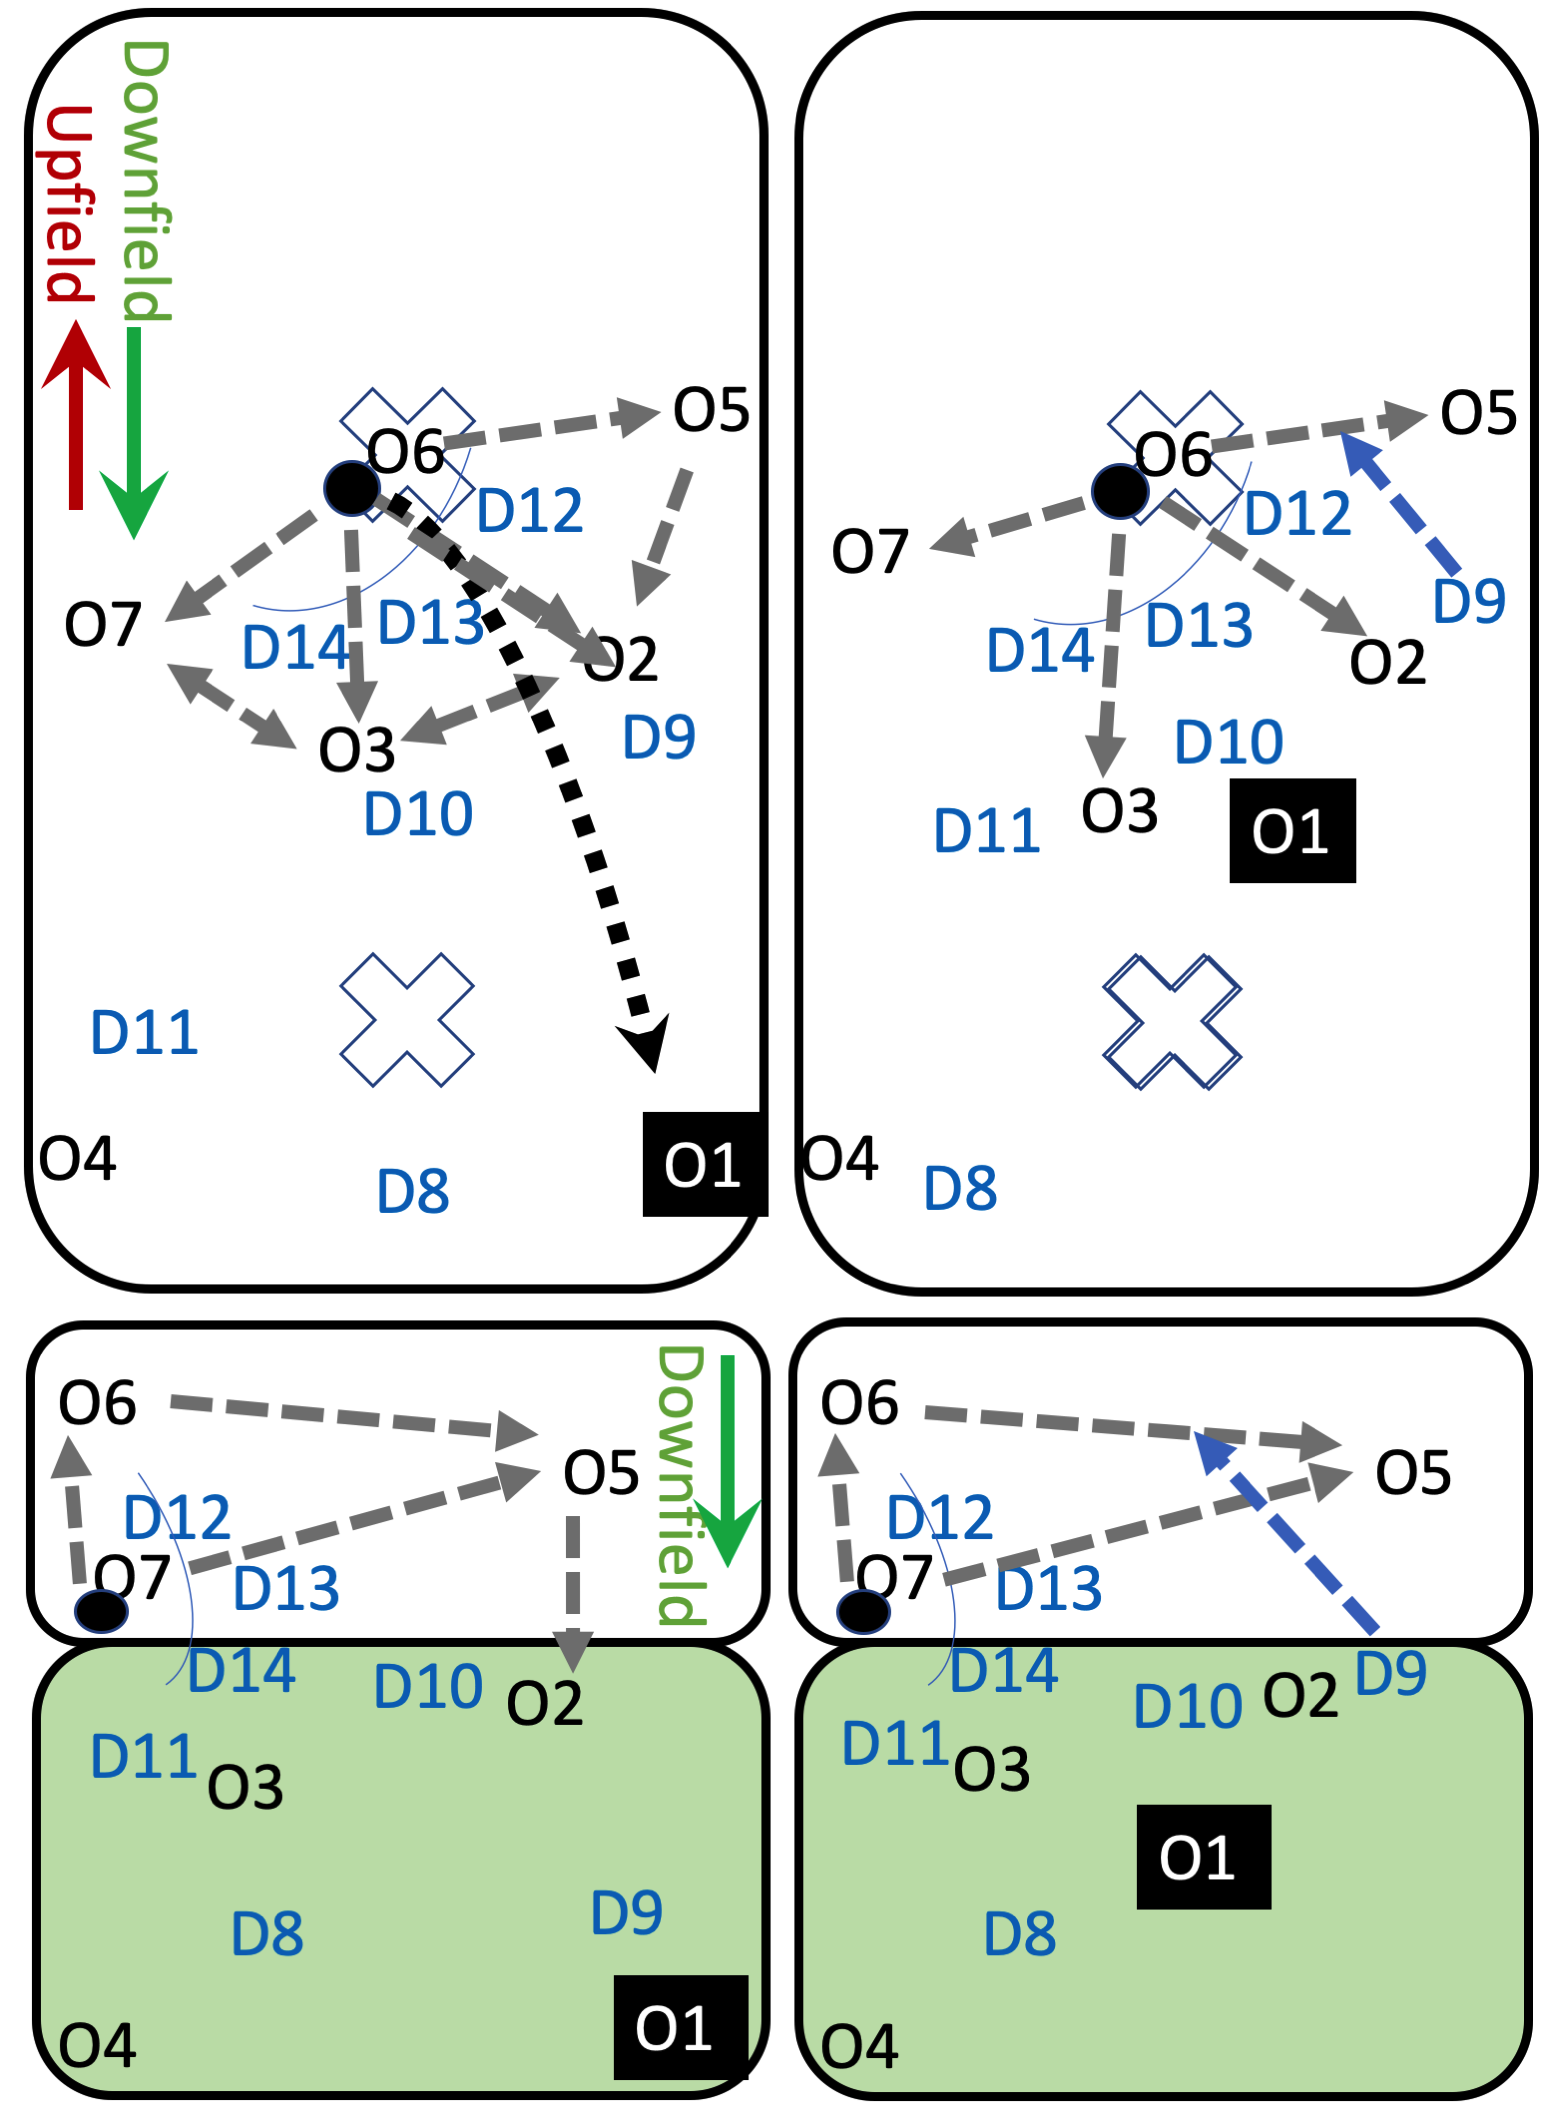
\includegraphics[width=\linewidth]{O1-zone331}
  \caption{331 zone formation}
  \label{fig:O1-zone331}
\end{marginfigure}

Figure \ref{fig:O1-zone331}
shows a 
3-3-1 zone, but
regardless of what it is,
the three ways to beat a zone are:
(1) over;
(2) round; or
(3) through. 
As O1 
(left wing), 
you are mostly relevant to 
(1) \smallcaps{over}, 
into the gap between 
D8 
and D9.
Figure \ref{fig:O1-zone331} shows 
throws from O6 to you 
(black dashed arrows):
(1) directly 
using a hammer
or a blade 
to get it there
as quickly as possible
or (2) throwing to A. 
If (grey arrows) 
O6 throws
over or through (to O2 or O3), 
or round (to O5) 
there are various ways 
that you, 
O5, 
O2, and
O3 
might seek to split
D10
and D9\footnote{
For example, 
O6 throws (2) through, 
to O2, 
who can then throw to 
O3, 
O5 
or you (O1).}
before the cup 
(D12-14) catch up. 
However, 
once the cup arrives, 
it is best to dump to O6, 
as otherwise 
you are trying to throw to 
one of 4-5 offensive players, 
covered by 7 defenders. 
Dump, 
then move downfield 
to make it 7-on-7 again.


\begin{marginfigure}%
  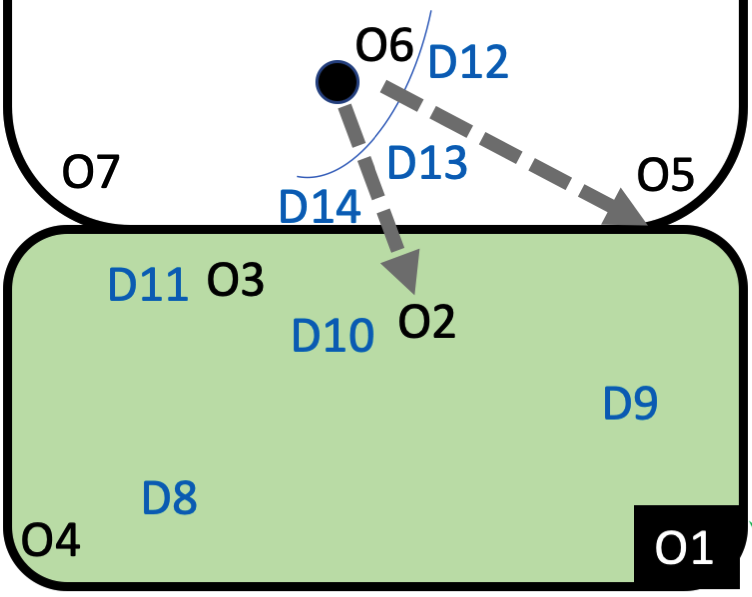
\includegraphics[width=\linewidth]{O1-zone331endzone}
  \caption{331 zone at endzone}
  \label{fig:O1-zone331endzone}
\end{marginfigure}

If the defence 
continues to play zone 
once the disc 
gets close to the endzone, 
you (O1) 
and the other wing (O4) 
can \smallcaps{go and stand 
on the back corners}
(Figure \ref{fig:O1-zone331endzone} left).  
The defence 
will then have to either 
leave you open
(a direct throw 
(1) over to you then scores)
or cover you
at the corner
(D8 
or D9), 
making more space 
for O2, 
O3, 
O5, 
O6 and
O7 
to score 
at the front of the endzone
The further 
you are from the back corner 
(Figure \ref{fig:O1-zone331endzone} right)
the more D8/9 
can cover both you
AND others,, 
and the harder 
it is to throw direct to you.
\end{document}
